\documentclass[english,,man]{apa6}
\usepackage{lmodern}
\usepackage{amssymb,amsmath}
\usepackage{ifxetex,ifluatex}
\usepackage{fixltx2e} % provides \textsubscript
\ifnum 0\ifxetex 1\fi\ifluatex 1\fi=0 % if pdftex
  \usepackage[T1]{fontenc}
  \usepackage[utf8]{inputenc}
\else % if luatex or xelatex
  \ifxetex
    \usepackage{mathspec}
  \else
    \usepackage{fontspec}
  \fi
  \defaultfontfeatures{Ligatures=TeX,Scale=MatchLowercase}
\fi
% use upquote if available, for straight quotes in verbatim environments
\IfFileExists{upquote.sty}{\usepackage{upquote}}{}
% use microtype if available
\IfFileExists{microtype.sty}{%
\usepackage{microtype}
\UseMicrotypeSet[protrusion]{basicmath} % disable protrusion for tt fonts
}{}
\usepackage{hyperref}
\hypersetup{unicode=true,
            pdftitle={A Simple, Dynamic Extension of Temporal Motivation Theory},
            pdfauthor={Christopher R. Dishop},
            pdfborder={0 0 0},
            breaklinks=true}
\urlstyle{same}  % don't use monospace font for urls
\ifnum 0\ifxetex 1\fi\ifluatex 1\fi=0 % if pdftex
  \usepackage[shorthands=off,main=english]{babel}
\else
  \usepackage{polyglossia}
  \setmainlanguage[]{english}
\fi
\usepackage{graphicx,grffile}
\makeatletter
\def\maxwidth{\ifdim\Gin@nat@width>\linewidth\linewidth\else\Gin@nat@width\fi}
\def\maxheight{\ifdim\Gin@nat@height>\textheight\textheight\else\Gin@nat@height\fi}
\makeatother
% Scale images if necessary, so that they will not overflow the page
% margins by default, and it is still possible to overwrite the defaults
% using explicit options in \includegraphics[width, height, ...]{}
\setkeys{Gin}{width=\maxwidth,height=\maxheight,keepaspectratio}
\IfFileExists{parskip.sty}{%
\usepackage{parskip}
}{% else
\setlength{\parindent}{0pt}
\setlength{\parskip}{6pt plus 2pt minus 1pt}
}
\setlength{\emergencystretch}{3em}  % prevent overfull lines
\providecommand{\tightlist}{%
  \setlength{\itemsep}{0pt}\setlength{\parskip}{0pt}}
\setcounter{secnumdepth}{0}
% Redefines (sub)paragraphs to behave more like sections
\ifx\paragraph\undefined\else
\let\oldparagraph\paragraph
\renewcommand{\paragraph}[1]{\oldparagraph{#1}\mbox{}}
\fi
\ifx\subparagraph\undefined\else
\let\oldsubparagraph\subparagraph
\renewcommand{\subparagraph}[1]{\oldsubparagraph{#1}\mbox{}}
\fi

%%% Use protect on footnotes to avoid problems with footnotes in titles
\let\rmarkdownfootnote\footnote%
\def\footnote{\protect\rmarkdownfootnote}


  \title{A Simple, Dynamic Extension of Temporal Motivation Theory}
    \author{Christopher R. Dishop\textsuperscript{1}}
    \date{}
  
\usepackage{color}
\usepackage{soul}
\usepackage{xcolor}
\definecolor{lightblue}{rgb}{0.90, 0.95, 1}
\sethlcolor{lightblue}

\shorttitle{GOAL SAMPLING}
\usepackage{lineno}

\linenumbers

\authornote{Christopher R. Dishop, Department of Psychology,
Michigan State University

Correspondence concerning this article should be addressed to
Christopher R. Dishop, 316 Physics Rd \#348, East Lansing, MI 48824.
E-mail:
\href{mailto:dishopch@msu.edu}{\nolinkurl{dishopch@msu.edu}}}

\abstract{
Steel and Konig's (2006) temporal motivation theory (TMT) has been
criticized for its static representation and neglect of the environment.
In this paper, I develop goal sampling theory (GST) to appease these
criticisms and extend our understanding of goal choices beyond momentary
preferences and into dynamic updating and global sampling behavior
across time. GST draws from temporal motivational theory (TMT), sampling
models of impression formation, and organizational theory on how the
environment constrains behavior and situates aspects of each into a
formal representation of goal sampling. Doing so addresses the
limitations of our prior thinking, introduces new concepts and
predictions, and provides a mathematical framework that lends itself to
computational modeling.


}

\usepackage{amsthm}
\newtheorem{theorem}{Theorem}[section]
\newtheorem{lemma}{Lemma}[section]
\theoremstyle{definition}
\newtheorem{definition}{Definition}[section]
\newtheorem{corollary}{Corollary}[section]
\newtheorem{proposition}{Proposition}[section]
\theoremstyle{definition}
\newtheorem{example}{Example}[section]
\theoremstyle{definition}
\newtheorem{exercise}{Exercise}[section]
\theoremstyle{remark}
\newtheorem*{remark}{Remark}
\newtheorem*{solution}{Solution}
\begin{document}
\maketitle

Employees often face multiple, conflicting goals as they complete their
work day. Core tasks, such as skill acquisition and networking
opportunities, projects, and reports flood employee experiences while
superficial demands, such as emails, meetings, and phone calls threaten
to emerge at any moment. In these environments, how do individuals
decide which goal to pursue? What process guides their goal sampling
behavior over time? Goal choice theories often evoke utility functions
(Keeney \& Raiffa, 1976; Steel \& König, 2006; Von Winterfeldt \&
Edwards, 1982) to explain this operation, such that employees choose
goal `A' over goal `B' to the extent that `A' produces greater utility.
These explanations are among the most actionable organizational theories
due to their concrete predictions (Miner, 1980; Van Eerde \& Thierry,
1996a), but they have largely focused on single, static equations that
neglect how the decision process updates and evolves alongside the
constraints of the environment (Busemeyer, Townsend, \& Stout, 2002;
Luce, 1995). Goal choice theories across psychology, economics, and
sociology largely agree on the necessary function parameters (Steel \&
König, 2006), therefore it is time to move beyond specifying a single
equation and build a theory that describes the dynamics of goal choice
updating.

In this paper I unpack goal sampling theory (GST), a theory of goal
choice that subsumes prior research and embeds the individual utility
function in a framework that makes both competing and complimentary
predictions. \hl{Its purpose is to extend work by }Steel and König
(2006)\hl{by adding elements that are currently missing in their theory but have been highlighted by other authors as critical aspects of goal choice. That is, utility functions (referred to hereafter as $U$ functions) are used as a starting point to build on and the theory presented here shows how they are only one piece to a larger goal decision framework.}

The following paper moves sequentially, rather than presenting the
entire theoretical framework upfront, to simplify the equations and
clearly specify what each aspect represents.
\hl{Immediately below, I identify what other researchers have presented as criteria for sound goal-choice theory -- the criteria will be used as a backdrop for the rest of the paper. I then discuss individual components before presenting GST in full.}

\hypertarget{crucial-aspects-for-theories-of-goal-choice}{%
\subsection{Crucial Aspects for Theories of Goal
Choice}\label{crucial-aspects-for-theories-of-goal-choice}}

\hl{How employees pursue goals in organizations has been an extensive research stream for many years and so a number of criteria have emerged concerning what components theories of goal choice must cover. First, goal pursuit is a dynamic process and so dynamics must be specified and represented in the theory }(Neal,
Ballard, \& Vancouver,
2017)\hl{. This component addresses the transition rules for utility as an individual moves through time. Specifically, there must either be some mechanism relating prior to current utility or argument for why utility is independent of its past at each moment. Second, the theory must discuss the environment }(Lord,
Diefendorff, Schmidt, \& Hall,
2010)\hl{. The environment is now a core element in goal-choice research}
(DeShon \& Gillespie, 2005; Unsworth, Yeo, \& Beck,
2014)\hl{ and organizational theory more broadly} (Johns,
2018)\hl{, and the idea stems from the common notion running through much of Simon's writing that to understand human behavior it is necessary to study the structure of goal-relevant objects in the environment }(Simon,
1981).\hl{ Third, goal choice theories must address how goals are prioritized }(DeShon
\& Rench,
2009)\hl{. Even if an agent can only choose one goal at a time, situations often contain multiple, at times conflicting goals and so some method of priority is required. Finally, }Neal
et al.
(2017)\hl{ argue that formal theories are necessary because verbal theories tend to be imprecise, easily misunderstood, or ambiguous with respect to dynamics}
(Vancouver, Wang, \& Li, 2018).

\hl{My argument is that temporal motivation theory covers some but not all of the aspects listed above. Specifically, it is formal and specifies how individual's prioritize multiple goals but is limited in its dynamics and how it represents the environment. The rest of the paper is devoted to briefly describing TMT and then discussing how it can be extended to cover the criteria. Ultimately this discussion will lead to the full framework, GST, and several discussed implications. }

\hypertarget{choosing-a-goal}{%
\section{Choosing a Goal}\label{choosing-a-goal}}

Goals refer to internal representations of desired states (Austin \&
Vancouver, 1996), and the organizational goal-decision literature is
concerned with how employees choose which goal to pursue. This notion is
distinct from goal-striving, which describes effort and performance
strategies usually in the pursuit of a single goal (for exceptions, see
Schmidt \& DeShon, 2007; Vancouver, Weinhardt, \& Schmidt, 2010).
Theories of goal choice and decision making are present in economics,
psychology, and sociology, and are nicely integrated by Steel and König
(2006). Their temporal motivation theory (TMT) incorporates hyperbolic
discounting, expectancy theory, cumulative prospect theory, and need
theory into an integrated \(U\) function that predicts goal choice. The
details of those theories are not crucial here, as each delivers a
variant of a utility equation, such that:

\begin{equation}
U = f(X_{theory})
\end{equation} \noindent where \(U\) represents utility, or a preference
for a certain goal, and \(X\) is a set of variables whose formal
representation depends on the theory. The set of variables, \(X\), is
not the focus of this paper so it will only be briefly described here.
Core variables in the set include expectancy, valence, and
deadline/outcome time. Expectancy refers to a subjective belief about
the likelihood of achieving a goal. Valence is how much an individual
values the outcome that follows goal attainment, and time in TMT refers
to when the outcome is received (how distant the reward is).
\hl{As stated in} Steel and König
(2006)\hl{, many fields use $U$ functions -- meaning some combination of expectancy, valence, and time to reward -- to predict goal choice, so I use $U$ as represented in TMT as a starting point to expand on.}

\hl{How does TMT and its representation of $U$ compare against the criteria? The theory is formal, so there is little ambiguity in how the different aspects combine to produce utility (for details on the actual function that describes how expectancy, valence, and time to outcome are combined see the original paper by }Steel
and König
(2006)\hl{). It also handles goal priority well. An agent who is confronted with multiple, competing goals selects the goal with the greatest utility. That is, if an agent's subjective utility for goal 'A,' as produced by some combination of expectancy, valence, and time to reward, is greater than his subjective utility for 'B,' he decides to act toward goal 'A.' This notion may be somewhat simple but it is nonetheless adequately specified in the theory.}

\hl{Where it is limited is in its ability to capture dynamics and the environment }(Kanfer
\& Chen,
2016)\hl{. That is, irrespective of how complicated the function of expectancy, valence, and time to reward becomes, dynamics and the environment are left unspecified. It is these two aspects that this paper uses as catalysts to expand on. }

\hypertarget{dynamic-updating}{%
\section{Dynamic Updating}\label{dynamic-updating}}

Beginning with dynamics, utility functions have been labeled as time
insensitive, static, and unable to capture dynamic effects (Baumeister,
Vohs, \& Oettingen, 2016; Kanfer, 1990; Luce, 1999). Steel and König
(2006) respond to calls for a dynamic representation in TMT by formally
including time as a variable in their \(U\) function such that positive
outcomes far removed, compared to those that are close, produce lower
utility. Incorporating deadlines is appropriate, but simply including
time as a variable does not make the equation dynamic. That is, when the
\(U\) function incorporates time to reward it is still expressed as:

\begin{equation}
U = f(X_{theory})
\end{equation} \noindent but a variable, \(T\), which is the amount of
time an individual perceives that he has until a deadline occurs and an
outcome is rewarded, is incorporated into the set of \(X\). Doing so
captures subjective time, but it does not represent the process over
time. To do so, we can change the equation to acknowledge two
assumptions: 1) that \(U\) can change over time

\begin{equation}
U_{t}
\end{equation} \noindent and 2) that \(U\) is a function of current
variables in the set of \(X\):

\begin{equation}
f(X_{theory})_{t}
\end{equation} \noindent which gives us the following when we combine
those ideas:

\begin{equation}
U_{t} = f(X_{theory})_{t}.
\end{equation} \noindent That is, utility at time four depends on the
set of variables in \(X\) at time four, but utility at time five can be
different from utility at time four.

We now have a description of utility over time, but this representation
is still not consistent with what researchers would consider dynamic
modeling (Busemeyer, 2018; Voelkle \& Oud, 2015). Utility, as presented
above, is memoryless, where any effects at time \(t\) disappear and are
replaced by new effects at time \(t+1\). Dynamic representations account
for the past, and there are many empirical examples where prior states
carry over into the future.
\hl{Goal discrepancy states show consistency over time} (DeShon \&
Rench, 2009) \hl{reflecting satiated behavior }(Simon,
1956)\hl{. State goal orientations demonstrate positive autoregressive effects }(Beck
\& Schmidt,
2013)\hl{. Expectancies retain self-similarity over time and goal utilities tend to have memory in the sense that they are correlated across time even in periods of known development and change such as adolescents moving through high school }(Chouinard
\& Roy, 2008; Schmidt \& Dolis, 2009).

We represent states with memory mathematically by using autoregressive
terms. The following:

\begin{equation}
U_{(t+1)} = b_0 U_{t}
\end{equation} \noindent expresses utility dynamically, where
\(U_{(t+1)}\) is utility at the next time point and \(b_0\) represents
the coefficient relating current to future utility, which formally
models self-similarity (Petris \& An, 2010).

\textbf{Strengths of Incorporating Dynamics} Adding this dynamic element
reveals additional strengths of GST. First, utility now has similarity
across time. Prior explanations and models that do not present utility
in this way assume that goal choices are independent at each moment and
any effects at time \(t\) disappear and are replaced by new ones at time
\(t+1\). Although you can describe processes over time in this way,
these explanations amount to no more than compiled snapshots of behavior
that miss the continual flow governing the system (Ilgen \& Hulin,
2000). Often, the prior behavior of a variable is important to its own
development -- incorporating autoregression presents a more realistic
model of utility.

Models that do not account for the past also imply that utility is
unconstrained across time. That is, utility at time \(t\) can jump to
high or low values at time \(t+1\) irrespective of its position at
\(t\). Although I have not seen a discussion about whether such behavior
is possible for utility, it would be inconsistent with how researchers
in empirical articles describe the variables in the set of \(X\) (Dreher
\& Bretz, 1991; Erez \& Isen, 2002).

\begin{quote}
\begin{quote}
\textbf{Proposition 1} Utility has self similarity across time, such
that a goal's utility at time \(t\) is positively related to its value
at \(t + 1\).
\end{quote}
\end{quote}

\hypertarget{the-environment}{%
\section{The Environment}\label{the-environment}}

\hl{The second extension is to incorporate the environment and thereby satisfy an additional criteria}
(Simon,
1992)\hl{. By environment, I do not mean individual subjective perceptions concerning workplace aspects such as climate, psychological safety, or leadership, but random, situational stimuli that impinge upon actors }(Cappelli,
1991)\hl{. This perspective is similar to the notion of shocks in the unfolding model of employee turnover in which discrete situations (e.g., a large company layoff) make some actions more likely than others }(Lee
\& Mitchell,
1994)\hl{, to events in affective events theory in which random stimuli, such as a computer crash or a coworker running late, cause changes in employee affect and subsequent behavior patterns }(Weiss
\& Cropanzano,
1996)\hl{, and to Simon's representation of environment in his simple rules model }(Simon,
1956)\hl{ in which by context he means some arrangement of goal-relevant objects. Applied to this paper, the idea is that the environment constrains which goals are available at any given moment }(Neal
et al., 2017).

Consider a few examples: An employee has a high utility for goal `A' but
is forced to work on goal `B' by her manager; A co-worker is sick and
asks another individual to cover his tasks for the day; Low performance
at a neighboring branch requires an individual to put off her current
work and help train her fellow employees; A Wi-Fi outage constrains an
individual's set of goal options; An email with a provocative subject
line draws an individual's attention away from his current goal. These
examples are simple but are by no means uncommon, yet they are difficult
to represent with only utility. Moreover, they reveal that some
environmental constraints are consistent but others are random or
difficult to predict. Instantiating this notion into a representation of
goal choice, therefore, can be done with likelihoods, where an
individual has a probability of choosing a goal at a given moment with
respect to the environmental constraints. Stated formally:

\begin{equation}
\Theta_{A} = E * U_{A}
\end{equation} \noindent where \(\Theta_{A}\) represents the likelihood
of choosing goal `A,' which is a function of both the environment,
\(E\), and the utility of `A', \(U_{A}\). If the environment restricts
goal `A' such that it cannot be sampled, then \(E\) would be zero and
the likelihood of choosing `A' would also become zero. Although this is
a simple representation of the environment, Meehl (1967) suggested
creating simple formulas such as the one presented despite an incomplete
understanding of the `true' function (see also Morgan \& Winship, 2015).
We may never be able to adequately capture the environment, but it is
important to represent nonetheless.

\textbf{Strengths of Incorporating the Environment} By specifying
equation two I reveal several strengths of GST that are missing in prior
work. First, prior utility models cannot account for situations like
those presented above where context forces an individual to change
goals. These models either assume that the environment does not matter
or is somehow incorporated into the variables that make up utility
(valence, expectancy, deadline time). This second assumption does work
occasionally -- if, for example, a government shutdown creates new
deadline times -- but it is not amenable to the spectrum of situations
described above.

Second, creating a likelihood function by combining the environment with
utility demonstrates GST's focus on probabilistic goal sampling rather
than a deterministic choice. Researchers use probabilistic terms to
describe valence and expectancy (Van Eerde \& Thierry, 1996b), but prior
formulae for choosing goals imply that two choices at different points
in time should be identical if the values in the set of \(X\) at each
are the same. GST, conversely, acknowledges that goal choices may differ
from one moment compared to another despite equal utility at both. The
environment term, therefore, acts like a mathematical error term and
captures the notion of different goal choices despite identical utility
across time. Probabilistic models are also increasingly popular because
even deterministic systems can create unpredictable behavior (Mitchell,
2009), GST therefore presents a model consistent with the broader
scientific literature.

\begin{quote}
\begin{quote}
\textbf{Proposition 2} Goal sampling at two time points may be different
-- even when utility is exactly the same -- because the environment
forces sampling.
\end{quote}
\end{quote}

\hl{Before moving on, it is helpful to reiterate what has been covered so far. With very simple extensions, TMT has been updated to cover additional criteria for goal-choice theories. Dynamics is represented by positing the utility term at $t + 1$ as a function of its value at $t$ and so the notion of state consistency, self similarity, and memory is embodied in the theory. Context is represented by including an additional term and multiplying it by utility so that the theory adequately captures situations in which the environment shuts off or ramps up utility for some goals but not others.}

\hl{At this point, I pivot and discuss one more extension that is important for goal choice but not directly tied to one of the four criteria that opened this paper: feedback from choosing a goal }(Kanfer,
Frese, \& Johnson,
2017)\hl{. Experiences people receive from pursuing goals is thought to be an important aspect underlying which goals they select in the future. When someone experiences performance ambiguity they are more likely to switch and pursue goals where performance feedback is made available }(Schmidt
\& DeShon,
2010)\hl{. People tend to allocate their time toward goals that provide them with immediate and specific hedonic feelings }(Northcraft,
Schmidt, \& Ashford,
2011)\hl{ or where they can receive the most information regarding what goal pursuit ultimately leads to }(Neal
et al.,
2017)\hl{. Choosing between an individual versus team goal is somewhat determined by the experiences an individual has with the other team members versus the satisfaction he receives from his individual task}
(Courtright, Thurgood, Stewart, \& Pierotti,
2015)\hl{. Finally, when an individual experiences greater positive affect for one goal compared to another her valence and expectancy for that goal tend to increase}
(Schmidt, Beck, \& Gillespie,
2012)\hl{. The theory presented here incorporates these effects through experience sampling, which is described next.}

\hypertarget{experience-sampling}{%
\section{Experience Sampling}\label{experience-sampling}}

GST claims that goal experiences, or subjective evaluations of the
feedback and rewards received from sampling a goal, combine with utility
and the environment to drive future goal sampling. The mechanism by
which this happens is drawn from Denrell's (2005; 2007) sampling model
of impression formation, where people are more likely to sample (i.e.,
engage with) others for whom they have positive impressions, but stop
sampling anyone for whom they have negative impressions. GST extends
this notion to goals and experiences with their outcomes. If an
individual receives a subjectively favorable experience from a goal then
its utility increases and the individual becomes more likely to sample
it again in the future. When goals produce unfavorable outcomes,
conversely, individuals stop sampling (with a certain probability).
Relating goal sampling to prior experiences not only facilitates a
dynamic understanding of the process, but it also captures the classic
effects of feedback and reward (Dickinson, 1989; Kerr, 1975; Ludvig,
Bellemare, \& Pearson, 2011; Pinsker, Kupfermann, Castellucci, \&
Kandel, 1970; Rescorla \& Wagner, 1972).

A formal representation of utility updating based on its own prior state
and the sampling experience is as follows:

\begin{equation}
U_{(t+1)} = b_0 U_{t} + b_1 P_t
\end{equation} \noindent where \(P_t\) represents the experience of a
goal at time \(t\), \(b1\) is the weight relating experience to utility,
and all other terms are defined above.

Utility then influences the probability of sampling alongside the
constraints of the environment at the next time point (\(E_{t+1}\)):

\begin{equation}
\Theta_{(t+1)} = E_{t+1} * {\frac {1}{1 + e^{U_{(t+1)}}}}
\end{equation} \noindent where \(\Theta_{(t+1)}\) represents the
likelihood of sampling at \(t+1\) and all other terms are defined above.
I will thoroughly discuss the components of these equations in later
sections. What is important here is to recognize that we mathematically
represented the following: utility and the goal sampling experience
influence utility at the next time point (equation 8), and at this time
utility combines with the environment to inform the likelihood of goal
sampling (equation 9).

\textbf{Strengths of Incorporating Experience Sampling} Incorporating
experience sampling provides two strengths beyond prior work. First, I
account for the known, classic effects of feedback and rewards. Second,
GST captures goal sampling irrespective of goal completion. There are
many examples where individuals can still sample goals even after
completing them, but past utility theories overlook these situations by
focusing only on behavior leading up to goal completion. These
implications, however, can be difficult to see from the equations; I
therefore discuss them with examples below.

GST predicts that goal experiences influence future goal sampling.
Again, an experience in GST is an individual's subjective evaluation of
the feedback or reward that a specific goal sample produces. For
example, imagine a professor setting the goal to read 50 pages of a
book. After one sample of this goal she receives feedback in
(potentially) many forms, such as pay, social acknowledgment from
others, or feelings regarding reading itself (e.g., pleasure or
exhaustion). GST summarizes her subjective evaluation of this feedback
with a single value: the experience. If taking action toward the `read
50 pages' goal results in a positive experience then the professor is
more likely to sample it again in the future. But if doing so produces a
negative experience then she has a much lower sampling probability. In
GST, therefore, the decision to sample is directly tied to utility and
the accumulated prior experiences on which it is based.

\begin{quote}
\begin{quote}
\textbf{Proposition 3} Goal choices at time \(t\) are positively related
to subjective evaluations of a goal experience at the immediately prior
time point \(t - 1\), such that individuals are more likely to sample
goals that provide a subjectively favorable experience at \(t - 1\) but
less likely to sample goals that provide a subjectively unfavorable
experience at \(t - 1\).
\end{quote}
\end{quote}

Second, GST focuses on global sampling behavior and the mechanism just
described applies irrespective of whether or not individuals complete
the goal. Rather, goal completion in GST is viewed as another experience
of sampling. To continue the example, imagine two situations: one where
the professor does \emph{not} complete her goal of reading 50 pages, and
a second where she does complete it. Both of these situations are
samples of the `50 pages' goal where future sampling depends on her
perceptions of the experience feedback at each sample.

Consider first the situation where she does \emph{not} complete the
goal. If she views this sample as negative because she underperforms,
then sampling the `50 pages' goal is unlikely moving forward. But if
other positive aspects of reading overwhelm the negative
underperformance, such as the riveting nature of the material or the
tranquility surrounding quiet reading time, then the probability of
future sampling is higher.

Turn now to the situation where she does complete the `50 pages' goal.
If she views this experience as negative (due to say, exhaustion), then
future sampling is lower than if she finds the experience positive (due
to completing the goal). GST, therefore, focuses on utility updating and
sampling behavior across time due to various experiences regardless of
where the individual lies on their `goal completion' continuum. If an
individual terminates a goal by completing it, then it can no longer be
sampled in the future. But there are many cases, the `read 50 pages'
being one, where goal completion does not remove the goal; GST captures
both of these situations.

\begin{quote}
\begin{quote}
\textbf{Proposition 4} The mechanism of goal sampling as presented in
GST is the same irrespective of whether or not the individual has
completed the goal.
\end{quote}
\end{quote}

\hypertarget{goal-sampling-theory}{%
\section{Goal Sampling Theory}\label{goal-sampling-theory}}

I have introduced important components for theories of goal choice.
Utility perceptions inform goal preferences in the moment, the
environment constrains which goals are available, and prior experiences
update goal sampling likelihoods. I discussed each individually to avoid
overwhelming the reader with equations, but I now move to the full goal
sampling theory and place these aspects into a `control structure'
framework to demonstrate how this process develops over time (Meehl,
1967; Newell, 1973).

In GST, goal choices are viewed as opportunities to sample goals.
Sampling results in an experience, which can be thought of as an
individual's subjective evaluation concerning the feedback or reward it
produces for that specific sample. This experience updates utility,
which then informs the likelihood of sampling that goal again in the
future -- alongside the constraints of the environment. Repeated
sampling is likely when prior experiences are positive and unlikely when
prior experiences are negative (Denrell, 2005), such that individuals
have a low probability of sampling goals that produced poor outcomes in
the past.

The core elements of the theory, therefore, include experiences,
utility, and goal sampling likelihoods. A goal is chosen to the extent
that it has a high likelihood and is made available by the environment,
its outcome then produces an experience for the individual, that
experience informs utility, and utility, finally, combines with the
environment to create the likelihood of sampling that goal again moving
forward. This mechanism integrates organizational (Kanfer, 2012),
environmental (Simon, 1956), sampling (Denrell, 2005), and decision
theory (Steel \& König, 2006) concepts that provide a fruitful
description of goal choices. Theories suffer, however, to the extent
that they cannot be expressed mathematically (Pearl, 2009), so I now
present a formal model that incorporates each component.

For simplicity, consider one individual and her sampling behavior of a
single goal, `A.' Sampling `A' produces experiences that, in this case,
are assumed to follow a normal distribution. Instantiating GST into a
formal model of goal `A' would be:

\begin{equation}
P_{At} \sim {N}(0,1)
\end{equation}

\begin{equation}
U_{A(t+1)} = 
  \begin{cases}
  b_0 U_{At} + b_1 P_{At}, & \text{if goal 'A' is chosen}\\
  b_0 U_{At}, & \text{otherwise}
  \end{cases}
\end{equation}

\begin{equation}
\Theta_{A(t+1)} = E_{t+1} * {\frac {1}{1 + e^{U_{A(t+1)}}}}
\end{equation}

Beginning with equation 10, \(P_{At}\) represents her experience of goal
`A' at time \(t\) and is assumed to follow a normal distribution with a
mean of zero and standard deviation of one. This representation
acknowledges that her experience of goal `A' can be positive, negative,
or neutral. Moving to equation 11, her utility of goal `A' at time
\(t+1\) (\(U_{A(t+1)}\)) is influenced by the experience of goal `A' (to
the degree of \(b_1\)) but only when she samples `A.' If she does not,
then the experience cannot happen and thus does not influence utility.
In both cases, her prior utility influences current utility to the
degree of \(b_0\). Equation 12 represents her likelihood of sampling
goal `A' at the next time point. The likelihood of sampling goal `A'
(\(\Theta_{A}\)) at \(t+1\) is a function of the environment
(\(E_{t+1}\)) and a power function of utility. If utility for goal `A'
is high, then sampling `A' is likely to the extent that the environment
is amenable to that choice. In GST, this process is assumed to operate
across all possible goals in the environment, which means that our
example individual would have a utility for each possible goal, and at
each moment she would act toward the goal with the greatest likelihood.

Simple mathematical representations are preferred over their complex
counterparts (Miller \& Page, 2009; Stewart, 2012), and the power
function, at first, seems unnecessary. I use it here because it has
empirical support (Guadagni \& Little, 1983; Yechiam \& Busemeyer,
2005), is present in Denrell's original social impression sampling model
(2005), and can handle negative values that emerge from equation 10.

One of the benefits of formal theories is that we can implement them as
computational models to ensure their behavior is appropriate. I
programmed equations 10 - 12 into a simple computational model where our
example employee chooses between two goals, `A' and `B', over 20 time
points. Figure one shows her utility for both goals across time. The top
of the graph shows which goal she chooses at each time by presenting the
letter `B' or `A' in boldface. For example, her sequence was `B,' `A,'
`B' for the first three time points, respectively. We can see that
utility demonstrates self similarity across time due to the
autoregressive parameter, \(b_0\) (set to 0.3 for both goals) and the
data are stationary. Moreover, she chooses the goal that has the
greatest utility at each respective time, therefore the framework -- and
its instantiation in a computational model -- produces consistent
behavior.

Although utility demonstrates self similarity over time, why do we do
see fluctuations in Figure one? These changes are due to her
experiences, which are shown with respect to her utility in Figure two.
The top panel reveals her experiences and utility across time for goal
`A,' whereas the bottom panel is the same but for goal `B.' Experiences
are bar plots because they are independent: her experience outcome at
time seven does not depend on her experience at time two. This figure
demonstrates the lag effect of experiences on utility. For example, her
experience of goal `B' at time one is negative (bottom panel), and this
drives her utility of goal `B' down at the next time point. Similarly,
she has a positive experience of goal `A' at time eight (top panel) and
this increases her utility of goal `A' at the next time point. Also
notice that she does not receive an experience value (i.e., she does not
experience) goal `A' at time points when she chooses goal `B' (and vice
versa).

In summary, GST unites the pieces I have discussed throughout this paper
and produces reasonable behavior when instantiated as a computational
model. Having introduced the theory as a whole, I can now turn to its
last few implications, implications that concern utility estimates,
their stability, and their reliance on experiences. Specifically, if we
think about experiences as being drawn from a distribution (equation 10)
then we need to consider how different draws inform utility. I will
explain these implications below with examples because, although we gain
advantages by specifying the functional form of relationships (McPhee \&
Scott Poole, 1981; Vancouver et al., 2018), digesting the equations can
be difficult without connecting them to the real world. After presenting
these last implications and propositions I state the theory's
assumptions and then close the paper.

\hypertarget{additional-implications}{%
\subsection{Additional Implications}\label{additional-implications}}

In GST individuals are assumed to have their own, true utility for each
goal. Their beliefs about the utility of a goal at any moment is an
estimate of this true utility value, and because utility estimates are
updated by experiences in GST, individuals may arrive at biased
estimates of utility if goal samples produce unrepresentative
experiences. There are a host of (potentially unknowable) factors that
determine whether goals produce positive or negative experiences, and
GST raises the idea that these may create sampling tendencies that, in
turn, produce biased estimates of utility. For example, imagine a call
center employee with the goal of raising \$1200 over the course of a day
(Shantz \& Latham, 2009). This goal has a utility for our employee that
is informed by the set of \(X\) (e.g., expectancy) and also her sampling
experiences. For simplicity, assume that her true utility of the goal
`raise \$1200' is 0.7 and that individual experiences of sampling it are
\(\sim {N}(0,1)\). Now assume that her first experience is poor (e.g.,
-0.2). According to GST, she is unlikely to sample it again (unless
forced to by the environment) and, in this case, her estimate of -0.2
represents a false negative. This is not a bias stemming from poor
judgement or miss-intent, rather it is one of limited information. She
only has one sample from which to base her estimate, so the probability
of that estimate being representative of actual utility is low, and it
is unlikely to be corrected because experiences are directly tied to
sampling through their influence on utility. GST therefore predicts that
more (rather than less) sampling leads to more accurate utility
estimates.

\begin{quote}
\begin{quote}
\textbf{Proposition 5} Greater goal sampling, compared to limited
sampling, produces more accurate estimates of utility.
\end{quote}
\end{quote}

If we reverse proposition five and consider how utility estimates
influence sampling behavior we arrive at the next prediction of GST:
negative estimates of utility (or low utility) will be more stable than
positive estimates (given no environmental coercion). If experiences are
negative than an individual's utility estimate is unlikely to change
over time because they stop sampling, whereas positive estimates lead to
more sampling and potential utility changes. At any moment, a goal that
used to result in favorable experiences could instead produce an
unpleasant experience, lower utility, and subsequently reduce the
probability of sampling that goal again. Negative utility estimates are
therefore characterized by limited sampling and stability, whereas
positive utility estimates are characterized by greater sampling and
instability (but no greater than allowed by \(b_0\)).

\begin{quote}
\begin{quote}
\textbf{Proposition 6} Negative utility estimates are more stable than
positive utility estimates because the latter lead to more goal sampling
and are therefore suspect to change.
\end{quote}
\end{quote}

Another implication of GST is that we are more likely to find a greater
amount of false negative utility estimates than false positives among
people who are free to sample goals. Again, positive experiences produce
more sampling, which allows an individual to come to a more accurate
representation of the experience distribution for a given goal and the
utility it can provide. When sampling does not occur, due to negative
experiences, improper utility estimates cannot be corrected over time.
False negatives are therefore likely to persist while false positives
are not.

Consider students in a graduate program who each have a goal of
analyzing two data sets, and assume all are, at first, freely allowed to
sample this goal as they please. After a period of time we would find a
distribution of utility estimates among our students and each would have
sampled the goal a different number of times. If we then forced every
student to sample the `two data set' goal repeatedly, GST predicts that
we would find more cases of people raising their utility estimates than
lowering it. This is not to say that there would be more instances of
positive utility. Rather, GST predicts a larger proportion of false
negatives in the pool of estimates in situations where sampling is tied
to utility and no environmental coercion exists (initially).

To unpack this notion even further, imagine that ten students have true
utility estimates of 0 for the `two data set' goal and all of their
experience distributions are also centered about 0. Again, we let the
students sample at will for a period of time. Students who initially
receive positive experiences sample the goal with greater frequency and
subsequently reduce their positive estimate toward 0 as they gather more
samples, whereas students with initially poor experiences stop sampling
and their estimates remain negative. When we return to force the
students to sample this goal, only the negative estimates can change
because the students with initially (false) positive estimates have
built a large number of samples centered about the true value.

\begin{quote}
\begin{quote}
\textbf{Proposition 7} There are greater amounts of false negative
utility estimates than false positives where individuals are free to
sample goals.
\end{quote}
\end{quote}

The examples used to describe propositions five through seven were
technical. Here is a summary example that is less abstract. Imagine an
employee who wants to be more friendly and therefore sets a goal to
spend 20 minutes casually speaking with people in a neighboring
department every other day. His first sample goes well. He felt immersed
in the conversation, learned about other employees, found them polite
and interesting, and ultimately believed that this sample of the goal
``20 minutes of casual speaking'' helped him become a bit more friendly.
These feelings and outcomes, in sum, represent his experience of this
specific sample. When he samples the goal again, however, he does not
have a good experience. Instead, he feels that he annoyed the others and
came off as a brown nose. This new experience then lowers his belief
about the ability of this ``casual speaking'' goal to make him more
friendly. As he continues to sample the goal his utility estimate
bounces around across time and his experiences accumulate into an
experience distribution. His utility estimate will be more accurate when
he converses with other employees many times and builds a large
experience distribution, compared to a situation where he only tries the
goal once or twice (proposition 5). Moreover, after several bad
conversation experiences his utility estimate will be low and he will be
unlikely to continue, which means that his utility estimate will not
change (proposition 6). Finally, if we expand this example to 100
employees who are free to sample the ``conversation'' goal we reach
proposition 7. GST predicts that, over time, there will be a greater
number of employees who falsely believe that the conversation goal is of
no utility compared to the number of employees who falsely believe that
the conversation goal is of great utility.

\hypertarget{assumptions-and-caveats}{%
\section{Assumptions and Caveats}\label{assumptions-and-caveats}}

Presenting GST's equations also makes a variety of assumptions clear.
First, this process is assumed to operate under conditions when sampling
is directly related to utility. In GST, the probability of goal sampling
cannot change without immediately prior utility perceptions changing
unless the environment forces sampling. There may be some situations,
however, where goal sampling is more or less sensitive to utility. In
these contexts, where various levels of sensitivity are important,
utility can be multiplied by an additional parameter in the likelihood
equation. Doing so is an unnecessary complication here, but future work
could certainly incorporate this additional parameter when needed.

Second, goal likelihoods are assumed to follow an exponential choice
rule (Luce, 1959). As stated, this equation was selected to remain
consistent with prior work, but a fruitful area for future research is
to determine environments where simpler functions are appropriate.

A number of assumptions are also embedded in how GST represents
experiences. GST assumes constant weighting of experiences on utility
across time (\(b_1\)) and this removes contrast effects. Of course, we
could also assume that \(b_1\) varies over time and thereby allow for
fluctuating weights. Moreover, GST assumes that positive and negative
experiences have the same effect on utility, and the implications of
breaking this assumption depend on whether we give positive or negative
experiences more weight. If positive experiences have a greater
influence than negative experiences, then utility bias would be lower
than cases where negative experiences have more weight because the
former situation favors greater sampling driven by positive experiences
and thus more representative estimates.

In its current form, GST does not capture primacy effects. In some
situations, the first experience may be so profound that it determines
all subsequent sampling and a formal representation of updating
likelihoods is not needed. These first impressions may then subsequently
produce self fulfilling prophecies and confirmation bias. These effects
should not be seen as irrelevant in GST, but are simply complimentary
mechanisms that emphasize different features.

Finally, GST assumes that experience distributions are independent from
goal utility estimates. Return to the `read 50 pages' goal example. GST
claims that experiences from sampling the goal `read 50 pages' inform
utility, and utility influences future sampling. GST does not, however,
directly tie utility to the outcome of the sampling experience. That is,
the professor's belief about her ability to perform the goal `read 50
pages' (or other aspects of utility) do not determine whether the
sampling experience is positive, negative, or neutral. There are many
components, some due to the professor and some not, that cause an
experience to be positive or negative, and although GST views these
experiences as important for utility updating across time it does not
necessarily make the reverse connection. It will be important for future
research to understand when utility informs the distribution of possible
experiences and when it does not.

\hypertarget{discussion}{%
\section{Discussion}\label{discussion}}

The main contributions of this article are as follows: (1) It develops a
dynamic model of goal sampling by extending work by Steel and König
(2006). As discussed throughout this paper, once dynamics is represented
in the equations a variety of implications emerge, but the core notion
is that utility retains something about itself through time; (2) It
presents an analytically tractable set of equations that are suitable
for computational modeling (Vancouver et al., 2018) and their
development helped satisfy the core goal-choice criteria; (3) The paper
establishes a link between several bodies of work, including
organizational theory and empirical work on the environment, sampling
models of biased impression formation, notions of dynamics and processes
over time, and the foundational utility aspects that formed the opening
of this paper.

\hl{Consider one final example on a topic that is relevant for sociology and organizational theory in which TMT and GST can be applied and then compared: navigating family and work relations}
(Allen, Johnson, Kiburz, \& Shockley, 2013; Blossfeld \& Huinink,
1991)\hl{. We will focus on one individual, Jeff, and his dual goals across work and family domains. At work, he has three goals: finish four reports by Friday, introduce himself to the new employee that now works in an adjacent office, and call his partner across the state, Karen, and discuss ideas for implementing a new employee training program. He also has three goals for his family life: attend his daughter's soccer game on Friday, spend time with his aunt who recently moved into town, and go fishing with his wife once a week. Each goal has a utility: Jeff has a belief about his ability to execute the actions necessary for goal completion (expectancy), a subjective value regarding the outcome he expects from each goal (value), and every goal has a time to reward, some more abstract than others. According to TMT and GST, he selects the goal with the greatest utility. Given this base structure, if we wiggle or perturb the situation }(Pearl
\& Mackenzie,
2018)\hl{ the differences between TMT and GST become apparent.}

\hl{First, consider a change meant to reveal the different perspectives on the environment. Imagine that Jeff's car breaks down on the way to work and he must sit at a rest stop for half of the day.}

\hypertarget{tmt.}{%
\subsubsection{TMT.}\label{tmt.}}

\hl{TMT predicts that utilities -- and therefore goal selection -- do not change in this scenario. Whichever goal had the greatest utility before the incident remains the top choice, and Jeff chooses to approach that goal. Jeff's self-efficacy toward each goal remains the same because his personal abilities and their capacity to execute actions did not undergo any changes. He still values the reward from spending time with his aunt in the same way that he did prior to having his car break down, and the same is true for his other goals. Moreover, the time to reward for every goal has not changed. Whichever goal had the greatest utility before the car trouble remains so, according to TMT. If speaking with the new employee had the greatest utility before this car event, then TMT predicts that Jeff will somehow choose that goal as he sits at the rest stop -- hopefully it is clear that directly speaking with the employee is impossible given his location. }

\hypertarget{gst.}{%
\subsubsection{GST.}\label{gst.}}

\hl{GST represents the car issue as an environmental disturbance. Jeff is now stuck at the rest area, so his utility for goals that cannot be pursued are driven downward. Most of his goals are now constrained: he cannot complete his reports without access to his computer, he is not in the vicinity of the new employee and cannot engage with him or her, his aunt is elsewhere, and fishing is not an available option. The only goal made available by the environment is calling his partner, Karen, and speaking with her on the phone. GST therefore predicts that Jeff will call Karen and speak about employee training programs as he waits. By incorporating an environment term, GST captures the notion of situation effects on goal availability.}

\hl{Second, consider a change meant to reveal differences in how the theories represent utility dynamics. Imagine that Jeff has the same goals as mentioned prior and he goes about his day without trouble (i.e., no car breakdown). Midday, he receives an email from a friend informing him that it is now legal to keep Walleye -- his favorite fish -- caught from the lake that he goes to with his wife. Previously, it was illegal for him to keep Walleye from the lake. His perceived value for that goal then increases, causing its utility to improve as well.}

\hypertarget{tmt.-1}{%
\subsubsection{TMT.}\label{tmt.-1}}

\hl{TMT represents this change in utility toward the fishing goal as independent of its past value. There is no connection from prior to current utility, so at each moment utility for a given goal can be infinitely greater or lower than its immediately prior value. It is as if expectancy, value, and time to reward produce utility, everything vanishes, and then at the next moment the cycle begins again.}

\hypertarget{gst.-1}{%
\subsubsection{GST.}\label{gst.-1}}

\hl{GST claims that utility perceptions are connected through time. Jeff's utility toward the fishing goal increases, but it increases relative to where it was at the immediately prior moment. Jeff has a history with the fishing goal and its utility has bounced around over time. Given the exciting email, utility bounces up but from where Jeff left it last. The history of utility as represented in the autoregressive term acts like a prior: when it is large and utility is self-similar it is difficult to move, whereas it is more volatile when the autoregressive term is small. Adding this element allows GST to incorporate dynamics.}

\hl{Finally, GST also emphasizes experience sampling such that Jeff is unlikely to sample goals that produce poor experiences irrespective of his expectancy, value, and time to reward perceptions. Adding this element aligns the theory with the variety of sampling biases discussed throughout Denrell and colleagues' work }(Denrell,
2008)\hl{ in which actions toward or away from an objective occur not because of cognitive errors in how those objectives are perceived but through simple sampling experiences that result in valenced impressions. Perhaps Jeff has a low utility estimate for the fishing goal because the last three times he went random circumstances created poor impressions. Poor experiences with the fishing goal drove utility down, so when Jeff receives the positive email about Walleye his utility estimate increases but not beyond its accumulated low value. }

\hypertarget{conclusion}{%
\section{Conclusion}\label{conclusion}}

GST begins with a value concerning the experience of sampling a goal, a
value that summarizes how an individual evaluates goal feedback at that
moment. In GST, experiences can be registered irrespective of goal
completion, and this captures cases where 1) goal sampling continues
even after goal completion and 2) individuals leave and return to goals
multiple times before completing them. Embedding experiences into GST
also helps align the theory with prominent findings early in
psychological research regarding rewards and their effects on choices
(Ludvig et al., 2011). After a single sample takes place, the experience
informs utility, but it does not do so alone in a static way where prior
utility perceptions have no influence on the system. Rather, the prior
behavior of utility constrains any future update, which is a simple idea
but acknowledges the crucial difference between static and dynamic
modeling (Kondrashov, 2016). Moreover, relating prior to current utility
emphasizes that utility perceptions continue (but potentially without
perfect carryover) even when goals remain ``unsampled'' for a period of
time. The likelihood of choosing a goal again in the future is then
determined by this updated utility value and the environmental
constraints that force or deter sampling. This sampling mechanism
provides an explanation for how goal choices update over time and makes
several predictions that lend themselves to computational modeling.

\begin{figure}
\centering
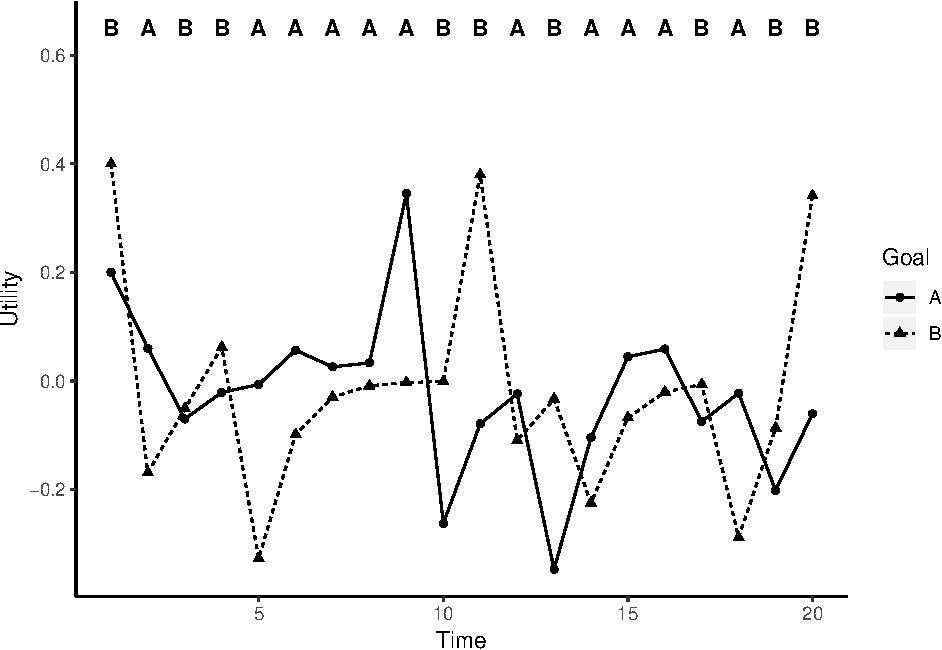
\includegraphics{figures/Figure1-1.pdf}
\caption{\label{fig:Figure1}Utility for goals \textbf{A} and \textbf{B} over
time. The letters at the top of the chart indicate which goal she chose
at each time.}
\end{figure}

\begin{figure}
\centering
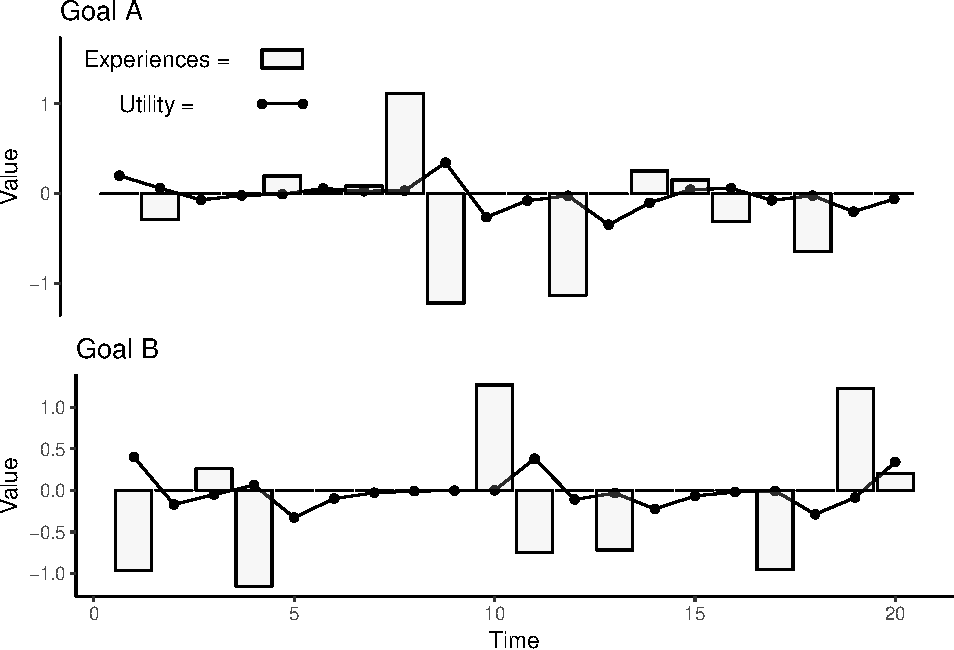
\includegraphics{figures/Figure2-1.pdf}
\caption{\label{fig:Figure2}The effect of experiences on utility across
time.}
\end{figure}

\newpage

\hypertarget{references}{%
\section{References}\label{references}}

\setlength{\parindent}{-0.5in}
\setlength{\leftskip}{0.5in}

\hypertarget{refs}{}
\leavevmode\hypertarget{ref-allen2013work}{}%
Allen, T. D., Johnson, R. C., Kiburz, K. M., \& Shockley, K. M. (2013).
Work--family conflict and flexible work arrangements: Deconstructing
flexibility. \emph{Personnel Psychology}, \emph{66}(2), 345--376.

\leavevmode\hypertarget{ref-austin1996}{}%
Austin, J. T., \& Vancouver, J. B. (1996). Goal constructs in
psychology: Structure, process, and content. \emph{Psychological
Bulletin}, \emph{120}(3), 338.

\leavevmode\hypertarget{ref-baumeister2016}{}%
Baumeister, R. F., Vohs, K. D., \& Oettingen, G. (2016). Pragmatic
prospection: How and why people think about the future. \emph{Review of
General Psychology}, \emph{20}(1), 3.

\leavevmode\hypertarget{ref-beck2013state}{}%
Beck, J. W., \& Schmidt, A. M. (2013). State-level goal orientations as
mediators of the relationship between time pressure and performance: A
longitudinal study. \emph{Journal of Applied Psychology}, \emph{98}(2),
354.

\leavevmode\hypertarget{ref-blossfeld1991human}{}%
Blossfeld, H.-P., \& Huinink, J. (1991). Human capital investments or
norms of role transition? How women's schooling and career affect the
process of family formation. \emph{American Journal of Sociology},
\emph{97}(1), 143--168.

\leavevmode\hypertarget{ref-busemeyer2018}{}%
Busemeyer, J. R. (2018). Old and new directions in strategy selection.
\emph{Journal of Behavioral Decision Making}, \emph{31}(2), 199--202.

\leavevmode\hypertarget{ref-busemeyer2002}{}%
Busemeyer, J. R., Townsend, J. T., \& Stout, J. C. (2002). Motivational
underpinnings of utility in decision making. \emph{Advances in
Consciousness Research}, \emph{44}, 197--220.

\leavevmode\hypertarget{ref-cappelli1991missing}{}%
Cappelli, P. (1991). The missing role of context in ob: The need for a
meso-level approach. \emph{Organizational Behavior}, \emph{13}, 55--110.

\leavevmode\hypertarget{ref-chouinard2008changes}{}%
Chouinard, R., \& Roy, N. (2008). Changes in high-school students'
competence beliefs, utility value and achievement goals in mathematics.
\emph{British Journal of Educational Psychology}, \emph{78}(1), 31--50.

\leavevmode\hypertarget{ref-courtright2015structural}{}%
Courtright, S. H., Thurgood, G. R., Stewart, G. L., \& Pierotti, A. J.
(2015). Structural interdependence in teams: An integrative framework
and meta-analysis. \emph{Journal of Applied Psychology}, \emph{100}(6),
1825.

\leavevmode\hypertarget{ref-denrell2005}{}%
Denrell, J. (2005). Why most people disapprove of me: Experience
sampling in impression formation. \emph{Psychological Review},
\emph{112}(4), 951.

\leavevmode\hypertarget{ref-denrell2008indirect}{}%
Denrell, J. (2008). Indirect social influence. \emph{Science},
\emph{321}(5885), 47--48.

\leavevmode\hypertarget{ref-deshon2005motivated}{}%
DeShon, R. P., \& Gillespie, J. Z. (2005). A motivated action theory
account of goal orientation. \emph{Journal of Applied Psychology},
\emph{90}(6), 1096.

\leavevmode\hypertarget{ref-deshon2009clarifying}{}%
DeShon, R. P., \& Rench, T. A. (2009). Clarifying the notion of
self-regulation in organizational behavior. \emph{International Review
of Industrial and Organizational Psychology}, \emph{24}, 217--248.

\leavevmode\hypertarget{ref-dickinson1989}{}%
Dickinson, A. M. (1989). The detrimental effects of extrinsic
reinforcement on ``intrinsic motivation''. \emph{The Behavior Analyst},
\emph{12}(1), 1--15.

\leavevmode\hypertarget{ref-dreher1991}{}%
Dreher, G. F., \& Bretz, R. D. (1991). Cognitive ability and career
attainment: Moderating effects of early career success. \emph{Journal of
Applied Psychology}, \emph{76}(3), 392.

\leavevmode\hypertarget{ref-erez2002}{}%
Erez, A., \& Isen, A. M. (2002). The influence of positive affect on the
components of expectancy motivation. \emph{Journal of Applied
Psychology}, \emph{87}(6), 1055.

\leavevmode\hypertarget{ref-guadagni1983}{}%
Guadagni, P. M., \& Little, J. D. (1983). A logit model of brand choice
calibrated on scanner data. \emph{Marketing Science}, \emph{2}(3),
203--238.

\leavevmode\hypertarget{ref-Ilgen2000}{}%
Ilgen, D. R., \& Hulin, C. L. (2000). \emph{Computational modeling of
behavior in organizations: The third scientific discipline.} American
Psychological Association.

\leavevmode\hypertarget{ref-johns2018advances}{}%
Johns, G. (2018). Advances in the treatment of context in organizational
research. \emph{Annual Review of Organizational Psychology and
Organizational Behavior}, \emph{5}, 21--46.

\leavevmode\hypertarget{ref-kanfermotivation}{}%
Kanfer, R. (1990). Motivation theory. In M. Dunnette \& L. Houghs
(Eds.), \emph{Handbook of industrial and organizational psychology}
(Vol. 1, pp. 124--151). Consulting Psychologists Press.

\leavevmode\hypertarget{ref-kanfer2012work}{}%
Kanfer, R. (2012). Work motivation: Theory, practice, and future
directions. In S. W. J. Kozlowski (Ed.), \emph{The oxford handbook of
organizational psychology} (Vol. 1, pp. 455--495).

\leavevmode\hypertarget{ref-kanfer2016motivation}{}%
Kanfer, R., \& Chen, G. (2016). Motivation in organizational behavior:
History, advances and prospects. \emph{Organizational Behavior and Human
Decision Processes}, \emph{136}, 6--19.

\leavevmode\hypertarget{ref-kanfer2017motivation}{}%
Kanfer, R., Frese, M., \& Johnson, R. E. (2017). Motivation related to
work: A century of progress. \emph{Journal of Applied Psychology},
\emph{102}(3), 338.

\leavevmode\hypertarget{ref-keeney1976}{}%
Keeney, R. L., \& Raiffa, H. (1976). \emph{Decision analysis with
multiple objectives: Preference and value tradeoffs}. Wiley\& Sons, New
York.

\leavevmode\hypertarget{ref-kerr1975}{}%
Kerr, S. (1975). On the folly of rewarding a, while hoping for b.
\emph{Academy of Management Journal}, \emph{18}(4), 769--783.

\leavevmode\hypertarget{ref-kondrashov_quantifying_2016}{}%
Kondrashov, D. A. (2016). \emph{Quantifying Life: A Symbiosis of
Computation, Mathematics, and Biology}. University of Chicago Press.

\leavevmode\hypertarget{ref-lee1994alternative}{}%
Lee, T. W., \& Mitchell, T. R. (1994). An alternative approach: The
unfolding model of voluntary employee turnover. \emph{Academy of
Management Review}, \emph{19}(1), 51--89.

\leavevmode\hypertarget{ref-lord2010self}{}%
Lord, R. G., Diefendorff, J. M., Schmidt, A. M., \& Hall, R. J. (2010).
Self-regulation at work. \emph{Annual Review of Psychology}, \emph{61},
543--568.

\leavevmode\hypertarget{ref-luce1959}{}%
Luce, R. D. (1959). \emph{Individual choice behavior: A theoretical
analysis}. New York: Wiley.

\leavevmode\hypertarget{ref-luce1995}{}%
Luce, R. D. (1995). Four tensions concerning mathematical modeling in
psychology. \emph{Annual Review of Psychology}, \emph{46}(1), 1--27.

\leavevmode\hypertarget{ref-luce1999}{}%
Luce, R. D. (1999). Where is mathematical modeling in psychology headed?
\emph{Theory \& Psychology}, \emph{9}(6), 723--737.

\leavevmode\hypertarget{ref-ludvig_primer_2011}{}%
Ludvig, E. A., Bellemare, M. G., \& Pearson, K. G. (2011). A primer on
reinforcement learning in the brain: Psychological, computational, and
neural perspectives. In \emph{Computational neuroscience for advancing
artificial intelligence: Models, methods and applications} (pp.
111--144). IGI Global.

\leavevmode\hypertarget{ref-mcphee_mathematical_1981}{}%
McPhee, R. D., \& Scott Poole, M. (1981). Mathematical modeling in
communication research: An overview. \emph{Annals of the International
Communication Association}, \emph{5}(1), 159--191.

\leavevmode\hypertarget{ref-meehl1967}{}%
Meehl, P. E. (1967). Theory-testing in psychology and physics: A
methodological paradox. \emph{Philosophy of Science}, \emph{34}(2),
103--115.

\leavevmode\hypertarget{ref-miller2009}{}%
Miller, J. H., \& Page, S. E. (2009). \emph{Complex adaptive systems: An
introduction to computational models of social life}. Princeton
university press.

\leavevmode\hypertarget{ref-miner1980}{}%
Miner, J. B. (1980). \emph{Theories of organizational behavior}. Dryden
Press.

\leavevmode\hypertarget{ref-mitchell2009}{}%
Mitchell, M. (2009). \emph{Complexity: A guided tour}. Oxford University
Press.

\leavevmode\hypertarget{ref-morgan2015}{}%
Morgan, S. L., \& Winship, C. (2015). \emph{Counterfactuals and causal
inference}. Cambridge University Press.

\leavevmode\hypertarget{ref-neal2017dynamic}{}%
Neal, A., Ballard, T., \& Vancouver, J. B. (2017). Dynamic
self-regulation and multiple-goal pursuit. \emph{Annual Review of
Organizational Psychology and Organizational Behavior}, \emph{4},
401--423.

\leavevmode\hypertarget{ref-newell1973}{}%
Newell, A. (1973). You can't play 20 questions with nature and win. In
W. G. Chase (Ed.), \emph{Visual information processing}. Academic Press.

\leavevmode\hypertarget{ref-northcraft2011feedback}{}%
Northcraft, G. B., Schmidt, A. M., \& Ashford, S. J. (2011). Feedback
and the rationing of time and effort among competing tasks.
\emph{Journal of Applied Psychology}, \emph{96}(5), 1076.

\leavevmode\hypertarget{ref-Pearl2009}{}%
Pearl, J. (2009). Causal inference in statistics: An overview.
\emph{Statistics Surveys}, \emph{3}, 96--146.

\leavevmode\hypertarget{ref-pearl2018book}{}%
Pearl, J., \& Mackenzie, D. (2018). \emph{The book of why: The new
science of cause and effect}. Basic Books.

\leavevmode\hypertarget{ref-petris2010r}{}%
Petris, G., \& An, R. (2010). An r package for dynamic linear models.
\emph{Journal of Statistical Software}, \emph{36}(12), 1--16.

\leavevmode\hypertarget{ref-pinsker1970}{}%
Pinsker, H., Kupfermann, I., Castellucci, V., \& Kandel, E. (1970).
Habituation and dishabituation of the gm-withdrawal reflex in aplysia.
\emph{Science}, \emph{167}(3926), 1740--1742.

\leavevmode\hypertarget{ref-rescorla1972}{}%
Rescorla, R. A., \& Wagner, A. R. (1972). A theory of pavlovian
conditioning: Variations in the effectiveness of reinforcement and
nonreinforcement. \emph{Classical Conditioning II: Current Research and
Theory}, \emph{2}, 64--99.

\leavevmode\hypertarget{ref-schmidtmotivation}{}%
Schmidt, A. M., Beck, J. W., \& Gillespie, J. Z. (2012). Motivation. In
I. B. Weiner, N. W. Schmitt, \& S. Highhouse (Eds.), \emph{Handbook of
psychology, industrial and organizational psychology} (Vol. 2, pp.
311--340). John Wiley \& Sons.

\leavevmode\hypertarget{ref-schmidt2007}{}%
Schmidt, A. M., \& DeShon, R. P. (2007). What to do? The effects of
discrepancies, incentives, and time on dynamic goal prioritization.
\emph{Journal of Applied Psychology}, \emph{92}(4), 928.

\leavevmode\hypertarget{ref-schmidt2010moderating}{}%
Schmidt, A. M., \& DeShon, R. P. (2010). The moderating effects of
performance ambiguity on the relationship between self-efficacy and
performance. \emph{Journal of Applied Psychology}, \emph{95}(3), 572.

\leavevmode\hypertarget{ref-schmidt2009something}{}%
Schmidt, A. M., \& Dolis, C. M. (2009). Something's got to give: The
effects of dual-goal difficulty, goal progress, and expectancies on
resource allocation. \emph{Journal of Applied Psychology}, \emph{94}(3),
678.

\leavevmode\hypertarget{ref-shantz2009}{}%
Shantz, A., \& Latham, G. P. (2009). An exploratory field experiment of
the effect of subconscious and conscious goals on employee performance.
\emph{Organizational Behavior and Human Decision Processes},
\emph{109}(1), 9--17.

\leavevmode\hypertarget{ref-simonant}{}%
Simon, H. (1981). The psychology of thinking: Embedding artifice in
nature. In H. Simon (Ed.), \emph{The sciences of the artificial} (pp.
63--73). MIT Press.

\leavevmode\hypertarget{ref-simon1956rational}{}%
Simon, H. A. (1956). Rational choice and the structure of the
environment. \emph{Psychological Review}, \emph{63}(2), 129.

\leavevmode\hypertarget{ref-simon1992explanation}{}%
Simon, H. A. (1992). What is an ``explanation'' of behavior?
\emph{Psychological Science}, \emph{3}(3), 150--161.

\leavevmode\hypertarget{ref-steel2006}{}%
Steel, P., \& König, C. J. (2006). Integrating theories of motivation.
\emph{Academy of Management Review}, \emph{31}(4), 889--913.

\leavevmode\hypertarget{ref-stewart2012}{}%
Stewart, I. (2012). \emph{In pursuit of the unknown: 17 equations that
changed the world}. Basic Books.

\leavevmode\hypertarget{ref-unsworth2014multiple}{}%
Unsworth, K., Yeo, G., \& Beck, J. (2014). Multiple goals: A review and
derivation of general principles. \emph{Journal of Organizational
Behavior}, \emph{35}(8), 1064--1078.

\leavevmode\hypertarget{ref-vancouver2018translating}{}%
Vancouver, J. B., Wang, M., \& Li, X. (2018). Translating informal
theories into formal theories: The case of the dynamic computational
model of the integrated model of work motivation. \emph{Organizational
Research Methods}, 1094428118780308.

\leavevmode\hypertarget{ref-vancouver2010}{}%
Vancouver, J. B., Weinhardt, J. M., \& Schmidt, A. M. (2010). A formal,
computational theory of multiple-goal pursuit: Integrating goal-choice
and goal-striving processes. \emph{Journal of Applied Psychology},
\emph{95}(6), 985.

\leavevmode\hypertarget{ref-van1996}{}%
Van Eerde, W., \& Thierry, H. (1996a). Vroom's expectancy models and
work-related criteria: A meta-analysis. \emph{Journal of Applied
Psychology}, \emph{81}(5), 575.

\leavevmode\hypertarget{ref-vaneerde1996}{}%
Van Eerde, W., \& Thierry, H. (1996b). Vroom's expectancy models and
work-related criteria: A meta-analysis. \emph{Journal of Applied
Psychology}, \emph{81}(5), 575.

\leavevmode\hypertarget{ref-voelkle2015relating}{}%
Voelkle, M. C., \& Oud, J. H. (2015). Relating latent change score and
continuous time models. \emph{Structural Equation Modeling: A
Multidisciplinary Journal}, \emph{22}(3), 366--381.

\leavevmode\hypertarget{ref-von1982}{}%
Von Winterfeldt, D., \& Edwards, W. (1982). Costs and payoffs in
perceptual research. \emph{Psychological Bulletin}, \emph{91}(3), 609.

\leavevmode\hypertarget{ref-weissaffective}{}%
Weiss, H. M., \& Cropanzano, R. (1996). Affective events theory: A
theoretical discussion of the structure, causes, and consequences of
affective experiences at work. In B. M. Staw \& L. L. Cummings (Eds.),
\emph{Research in organizational behavior} (pp. 1--74). Elsevier
Science.

\leavevmode\hypertarget{ref-yechiam2005}{}%
Yechiam, E., \& Busemeyer, J. R. (2005). Comparison of basic assumptions
embedded in learning models for experience-based decision making.
\emph{Psychonomic Bulletin \& Review}, \emph{12}(3), 387--402.


\end{document}
